\documentclass[aspectratio=169,t]{beamer}
\usepackage[utf8]{inputenc}
\usepackage[T1]{fontenc}
\usepackage[english]{babel}
\usepackage{hyperref}
\usepackage{tikz}

\usepackage{graphicx}
\usepackage{epstopdf}
\usepackage{multirow}

\usepackage{psfrag}
\usepackage{pgfplots}
\usepackage{framed}
\usepackage{xcolor}
\usepackage{booktabs}
\usepackage{caption}
\usepackage{epstopdf}
\usepackage{amsmath}
\usepackage{tabularx}
\usepackage[]{bookmark}
%\usepackage[3D]{movie15}
%\usepackage{media9}
\usepackage[binary-units,abbreviations]{siunitx}
\usepackage[textfont=normalsize, labelfont=normalsize, justification=centering]{subcaption}
\usepackage{marvosym}
\usepackage{calc}
\usepackage{color, colortbl}
\usepackage[]{svg} 
\usepackage[]{trfsigns} 
\usepackage[nomessages]{fp}
\usepackage[]{csquotes}\MakeOuterQuote{"}
\usepackage{tabto}
\selectcolormodel{rgb}

\makeatletter
\def\beamer@calltheme#1#2#3{\def\beamer@themelist{#2}
	\@for\beamer@themename:=\beamer@themelist\do
	{\usepackage[{#1}]{\beamer@themelocation/#3\beamer@themename}}}
\def\usefolder#1{\def\beamer@themelocation{#1}}
\def\beamer@themelocation{}
\usefolder{theme}

\usetikzlibrary{matrix,
	decorations.pathreplacing,
	calc,
	positioning,
	external,
	3d,
	shapes,
	arrows,
	pgfplots.statistics}
\pgfplotsset{compat=1.16}
\tikzstyle{faunode}=[rounded corners, draw=faublue, fill=faublue!10,  align=center, inner sep=0.3cm, line width=0.4mm]
\tikzstyle{fauellipseFixedWidth}=[ellipse, draw=faublue, fill=faublue!10,  align=center, inner sep=0.3cm, line width=0.4mm, minimum width=3cm]
\tikzstyle{fauellipse}=[ellipse, draw=faublue, fill=faublue!10,  align=center, inner sep=0.3cm, line width=0.4mm]
\tikzstyle{fauarrow}=[draw=faublue,->, line width=0.4mm]
\tikzstyle{fauline}=[draw=faublue, line width=0.4mm]


\usepackage[backend=bibtex,sorting=none,doi=true,style=phys]{biblatex}
%\usepackage[]{biblatex}
\bibliography{./references}

% Themes:
%  - fau:          FAU theme
%  - fau-tf:       TechFak FAU theme
%  - fau-tf-lme:   TechFak LME FAU theme
%
% Options:
%  - image:        Cover image on title page
%  - plain:        Plain title page
%  - longtitle:    Title page layout for long title
\usetheme[longtitle]{fau-tf-lme}

% END of THEME SETTINGS
% --------------------------------------------------------------------------------------------------------------------------------------------------------------------------

\sisetup{
exponent-product =\ensuremath{{\,\cdot\,}}
}

% Enable semi-transparent animation preview
\setbeamercovered{transparent}
\setbeamertemplate{blocks}[rounded]
\captionsetup{labelformat=empty,labelsep=none, labelfont=normalsize, justification=centering}


\newcommand\Wider[2][1.0cm]{%
\makebox[\linewidth][c]{%
  \begin{minipage}{\dimexpr\textwidth+#1\relax}
  \raggedright#2
  \end{minipage}%
  }%
}


\let\origitem\item
\renewcommand{\item}{\normalfont\origitem}
\newcommand{\bluefat}[1]{\textcolor{faublue}{\textbf{#1}}}
\newcommand{\bolditem}{\normalfont\origitem\bfseries}
\newcommand{\question}{{\bf Question: }}
\newcommand{\answer}{{\bf Answer: }}
\newcommand{\myExample}{{\bf Example }}
\newcommand{\real}{\mbox{${\mathbb R}$}}
\definecolor{defColor}{rgb}{0.8,0.87,0.97}
\definecolor{defColorT}{rgb}{0,0,0}
\definecolor{defColorF}{rgb}{1,1,1}
\newenvironment{myDefinition}{%
	\def\FrameCommand{\fboxsep=\FrameSep{} \fcolorbox{defColorF}{defColor}}%
	\color{defColorT}\MakeFramed{\FrameRestore{}}}%
{\endMakeFramed}

% Title page
\title[Medical Engineering II]{Medical Engineering - Imaging Systems}

\author{Prof.\ Dr. Bernhard Kainz \and Prof.\ Dr. Florian Knoll}
\date{SS 2023}
\institute{IDEA Lab and Computational Imaging Lab at Dept. AIBE}

\newcommand{\password}{\texttt{mt2\_ss22}}


\AtBeginSection[]{
	{
		\setbeamertemplate{footline}{}
		\begin{frame}[noframenumbering]{\insertsubtitle}
			 \tableofcontents[currentsection]
		\end{frame} 
	}
}
\AtBeginSubsection[]{
	{

		\setbeamertemplate{footline}{}
		\begin{frame}[noframenumbering]{\insertsubtitle}
			 \tableofcontents[currentsection, currentsubsection]
		\end{frame} 
	}
}


\subtitle{Motivation}


%TODO: add image sources

\begin{document}
\nocite{*}

\frame[plain,c]{\titlepage} % plain-Option deaktiviert Kopf- und Fusszeile

\begin{frame}
	\frametitle{We are\ldots}
	\begin{itemize}
		\setlength\itemsep{0.5cm}
		\item Image Data Exploration and Analysis (IDEA) and Computational Imaging lab
		      \begin{itemize}
			      \item \url{https://idea.tf.fau.eu/}
			      \item \url{https://www.cil.tf.fau.de/}
			      \item Werner-von-Siemens Strasse 61
		      \end{itemize}
		\item Lecturer: Prof.\,Dr.\ Bernhard Kainz
		\item Lecturer: Prof.\,Dr.\ Florian Knoll
		\item Exercise/Project Organization
		      \begin{itemize}
			      \item Marc Vornehm
		      \end{itemize}
		\item Contact: \texttt{\url{https://www.studon.fau.de/studon/goto.php?target=frm_4685856}}
	\end{itemize}
\end{frame}

\begin{frame}
	\frametitle{Medical Engineering II}
	\begin{block}{Aims of lecture}
		\begin{itemize}
			\item Show interesting applications
			\item Present important fundamentals and relate them to practical
			      implementation
		\end{itemize}
	\end{block}
	\begin{block}{Aims of exercises and project work}
		\begin{itemize}
			\item Implement methods from the lecture
			\item Deepen understanding
			\item Learn foundations of medical image processing
			\item Learn how to develop ImageJ Plugins
		\end{itemize}
	\end{block}
\end{frame}

\begin{frame}
	\frametitle{Medical Engineering II}
	\begin{columns}[c, onlytextwidth]
		\begin{column}{0.6\textwidth}
			\begin{block}{Lecture notes}
				\begin{itemize}
					\item Available as open access book: \url{https://www.springer.com/la/book/9783319965192}
					\item If you suspect an error, please write to the authors!
				\end{itemize}
			\end{block}
			\begin{block}{University code of conduct}
				\begin{itemize}
					\item Do not call in sick for the lecture or exercise
					\item Attendance is not mandatory
					\item Deadlines are strict
					\item You are responsible for your own success!\newline $\rightarrow$ We are only signposts!
				\end{itemize}
			\end{block}
		\end{column}\begin{column}{0.3\textwidth}
			\href{https://www.springer.com/la/book/9783319965192}{\includegraphics[width=0.9\textwidth]{Bilder/book_cover.png}}
		\end{column}
	\end{columns}
\end{frame}

\begin{frame}[c]{Lectures}
	\begin{itemize}
		\setlength\itemsep{0.4cm}
		\item \textbf{Hybrid mode}
		\item Lecture is in English
		\item Lecture Recordings in English: \href{https://www.fau.tv/course/id/2150}{https://www.fau.tv/course/id/2150 on FAU.tv}
		\item Lecture Recordings in German: \href{https://www.fau.tv/course/id/1022}{https://www.fau.tv/course/id/1022 on FAU.tv}
		\item Friday 12:15 c.t. - 13:45 on \href{https://teams.microsoft.com/l/team/19\%3adRCxup9jUsjM31xr9T4jdAFDB-ImEk_lU5Fy05ijYx81\%40thread.tacv2/conversations?groupId=6b2df36b-cec0-46b3-83d2-b4e6d1c6ac30\&tenantId=b2efcef3-8496-40b8-9de8-f135982f3461}{MS Teams}
		\item MS Teams channel password: \textbf{z2qebxs}
		\item Suggested consumption mode: hybrid + recordings 
		\begin{enumerate}
			\item sign up for class attentance on studon if you want to join in person (limited 30 places per week)
                        \item join on MS Teams live otherwise
			\item ask questions in the \href{https://www.studon.fau.de/studon/goto.php?target=frm_4685856}{Forum}
			\item we will discuss each week's content during Friday's lecture slot.   
		\end{enumerate}
	\end{itemize}
\end{frame}

%\iffalse
\begin{frame}[c]{Grading}
	\begin{itemize}
		\setlength\itemsep{0.4cm}
		\item No exam -- Grading of project work
		\item Condition of admission to project work:\\
		      Requirement: 50\% of all exercise points
		\item Do not copy:
		      \begin{itemize}
			      \item Automatic checks
			      \item Plagiarism leads to
			            \begin{itemize}
				            \item 0 points in exercise
				            \item grade 5.0 (not passed) in project work
			            \end{itemize}
			      \item for both!
		      \end{itemize}
		\item Work independently!
	\end{itemize}
\end{frame}

\begin{frame}[c]{Syllabus}
\begin{table}[]
\begin{tabular}{rll}
\multicolumn{1}{l}{Date} & \multicolumn{1}{l}{Topic}      & \multicolumn{1}{c}{} \\
21.04.23                 & Introduction                   &                      \\
28.04.23                 & System theory 1+2              &                      \\
05.05.23                 & System theory  3+4             &                      \\
12.05.23                 & Image Analysis                 &                      \\
19.05.23                 & Endoskopy, Microscopy 1       &                      \\
26.05.23                 & Microscopy 2, Ultrasound       &                      \\
02.06.23                 & no lecture                &                      \\
09.06.23                 & no lecture                      &                      \\
16.06.23                 & magnetic resonance imaging 1+2       &                      \\
23.06.23                 & X-Ray 1+2  &                      \\
30.07.23                 & CT 1                           &                      \\
07.07.23                 & CT 2                           &                      \\
14.07.23                 & Nuclear Medicine                         &                      \\
21.07.23                 & OCT          &                     
\end{tabular}
\end{table}
\end{frame}

\begin{frame}
	\frametitle{Project Work}
	\begin{itemize}
		\item Scientific working in the field of medical engineering
			\begin{itemize}
				\item Task: solve a problem of medical engineering
			\end{itemize}
		\item Consists of three parts:
			\begin{enumerate}
				\item Writing of a scientific report
				\item Practical: programming an ImageJ plugin in Java
				\item Short oral presentation in English
			\end{enumerate}
		\item Organization
			\begin{itemize}
				\item Project work spread over the whole semester
				\item Each student works on the project individually
				\item Duration: complete project work due by end of semester 
			\end{itemize}
	\end{itemize}
\end{frame}

\begin{frame}
	\frametitle{Exercise Sheets}
	\begin{block}{Organization}
		\begin{itemize}
			\item New exercise sheet every two weeks
			\item Each exercise sheet consists of two parts:
				\begin{enumerate}
					\item Theoretical and practical questions/tasks (deadline: two weeks)
					\item Project work -- will be published after last exercise, ETA 20.06 (deadline: end of
						semester)
				\end{enumerate}
		\end{itemize}
	\end{block}
	\vspace{-\bigskipamount}
	\begin{center}
	\alert{Start working on your project early!
		Do not wait until the end of the
		semester!}
\end{center}
%		\begin{block}{Submission of exercises}
%			\begin{itemize}
	%			\item Submission via EST  -- keep the deadlines in mind!
					
	%				\centering\url{http://est.informatik.uni-erlangen.de}
%			\end{itemize}
%		\end{block}
\end{frame}


\begin{frame}{Evaluation}
	\begin{itemize}
		\setlength\itemsep{0.3cm}
		\item All lectures and exercises at the school of engineering are evaluated
		\item Evaluations
		      \begin{itemize}
			      \item are anonymous
			      \item can only be done by participants of the lecture via TAN
		      \end{itemize}
		\item Evaluation as high impact on teaching
		      \begin{itemize}
			      \item Lecturer
			      \item Future students
			      \item You
		      \end{itemize}
	\end{itemize}
\end{frame}

\iffalse
\begin{frame}
	\frametitle{Important Password}
	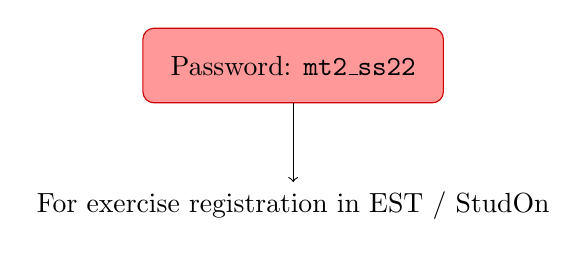
\begin{tikzpicture}
		\matrix [matrix of nodes, draw=red!80!black, fill=red!40!white, rectangle, rounded corners,
			align=left, inner sep=5pt]
		(m) {
			%			Login: mt1617\\
			Password: \texttt{\password}\\};
		%		\draw [decorate, decoration={brace, amplitude=10pt}, xshift=2em] ($(m.north
		%		east)+(2em,0)$) --
		%		($(m.south east)+(2em,0)$) node [midway, xshift=1em, anchor=west] {For lectures slides and notes};
		\node [below= of m] (t) {For exercise registration in EST / StudOn};
		\draw [->] (m) -- (t);
	\end{tikzpicture}

	\begin{center}
		\alert{\url{https://www.studon.fau.de/studon/goto.php?target=frm_4286923}}
	\end{center}
\end{frame}
\fi

\section{Introduction}

%TODO: check images
\begin{frame}[c]{Why do we need images?}

	\begin{columns}[c]
		\begin{column}{0.4\textwidth}

			\begin{itemize}
				\item Medical problems:
				      \begin{itemize}
					      \item fracture?
					      \item lesion?
					      \item perfusion?
					      \item metabolism?
					      \item atrophy?
					      \item and much more
				      \end{itemize}
			\end{itemize}
		\end{column}\begin{column}{0.5\textwidth}
			\begin{tabular}{cc}
				\includegraphics[width=.45\textwidth]{images/parallel_full.png}                                                               & \includegraphics[width=.45\textwidth]{images/155_13.jpg} \\
				\includegraphics[width=.45\textwidth, trim={0,  6cm, 0, 6cm},clip]{images/Communitive_midshaft_humeral_fracture_callus.jpg} &
				\includegraphics[width=.45\textwidth,trim={0,  4.7cm, 0, 0},clip]{images/appB.png}% \includegraphics[width=.45\textwidth]{images/Angiography_Superficial_Montage.png}
			\end{tabular}
		\end{column}
	\end{columns}
	%\begin{minipage}{0.4\linewidth}
	%\begin{figure}[htbp]
	%\raggedleft \includegraphics[width=.5\linewidth]{Bilder/gehirn2}
	%\end{figure}
	%\end{minipage}

	%\begin{minipage}{0.4\linewidth}
	%\end{minipage}
\end{frame}

\begin{frame}
	\frametitle{Imaging Modalities}

	\begin{figure}[htpb]
		\begin{center}
			\begin{tikzpicture}[scale=0.85, transform shape]

				\node (book) [] at (0,0) {\includegraphics[width=0.15\linewidth]{Bilder/book_cover.png}};
				\node (xray) [above=of book, fauellipseFixedWidth]  {X-ray};
				\node (ct) [above right=0.1cm and 1.0cm of book, fauellipseFixedWidth]  {CT};
				\node (oct) [ right =1.3cm of book, fauellipseFixedWidth]  {OCT};
				\node (mr) [below right = 0.3cm and 0.8cm of book, fauellipseFixedWidth]  {MR};
				\node (pet) [below left =0.3cm and 0.5cm of book, fauellipseFixedWidth]  {PET/SPECT};
				\node (us) [left =1.3cm of book, fauellipseFixedWidth]  {Ultrasound};
				\node (endo) [above left=0.3cm and 0.7cm of book, fauellipseFixedWidth]  {Endoscopy};

				\path[draw=faublue,->,line width=0.4mm] (book) -- (xray) node[midway, above right] {};
				\path[draw=faublue,->,line width=0.4mm] (book) -- (ct) node[midway, above right] {};
				\path[draw=faublue,->,line width=0.4mm] (book) -- (oct) node[midway, above right] {};
				\path[draw=faublue,->,line width=0.4mm] (book) -- (mr) node[midway, above right] {};
				\path[draw=faublue,->,line width=0.4mm] (book) -- (pet) node[midway, above right] {};
				\path[draw=faublue,->,line width=0.4mm] (book) -- (us) node[midway, above right] {};
				\path[draw=faublue,->,line width=0.4mm] (book) -- (endo) node[midway, above right] {};
			\end{tikzpicture}
		\end{center}
		%\caption{}
		%\label{fig:}
	\end{figure}


	%\begin{figure}[htbp]
	%\begin{center}
	%\includegraphics[width=.8\linewidth]{Bilder/imagingmodalities}
	%\end{center}
	%\end{figure}
\end{frame}


\section{Endoscopy}

\begin{frame}[c]{Endoscopy}

	Endoscopy \href{https://youtu.be/DUVDKoKSEkU}{https://youtu.be/DUVDKoKSEkU}

	Laparoscopy \href{https://youtu.be/sGtWyKZZhGE}{https://youtu.be/sGtWyKZZhGE}
	\begin{columns}[t, onlytextwidth]
		\begin{column}{0.5\textwidth}

			\begin{figure}
				\includegraphics[width=.9\linewidth]{images/stereo1.jpg}
				%\caption{Stereo Endoscopy}
			\end{figure}
		\end{column}\begin{column}{0.5\textwidth}
			\begin{figure}
				%\includegraphics[width=.8\linewidth]{Bilder/endoscopy2}
				%\vspace*{.25cm}
				\includegraphics[width=.9\linewidth]{images/sigma.png}
			\end{figure}
		\end{column}
	\end{columns}
\end{frame}


\section{X-ray}

%\begin{frame}[c]{X-Ray}
%\begin{columns}[c, onlytextwidth]
%\begin{column}{0.55\textwidth}
%\centering{}
%\includegraphics[width=\textwidth]{../mt1-script/Siemens_Images/XP/sm11359_SP_03.jpg}
%\end{column}\begin{column}{0.45\textwidth}
%\centering{}
%\includegraphics[height=0.95\linewidth]{../mt1-script/xray/images/Albert_von_Koelliker_hand.jpg}
%\end{column}
%\end{columns}

%%\begin{figure}

%%%file:///localhome/seitz_local/projects/MT1-lecture/
%%%file:///localhome/seitz_local/projects/MT1-lecture/mt1-script/xray/images/x-ray_tube.jpg
%%\end{figure}
%\end{frame}

\begin{frame}[c]{X-Ray}
X-Ray: \href{https://youtu.be/GRdq8gXeDA4}{https://youtu.be/GRdq8gXeDA4}
\begin{columns}[c, onlytextwidth]
  \begin{column}[c]{0.55\textwidth}
		\centering{}
		\includegraphics[height=0.8\textheight]{images/Albert_von_Koelliker_hand.jpg}
	\end{column}\begin{column}{0.45\textwidth}
		\centering{}
		\includegraphics[height=0.4\textheight]{Bilder/Roentgen-Roehre}\\ %\\[0.4cm]
		\includegraphics[height=0.4\textheight]{images/x-ray_tube.jpg}
	\end{column}
\end{columns}

%%\begin{figure}

%%%file:///localhome/seitz_local/projects/MT1-lecture/
%%%file:///localhome/seitz_local/projects/MT1-lecture/mt1-script/xray/images/x-ray_tube.jpg
%%\end{figure}
\end{frame}

\section{Angiography}

\begin{frame}[c]{Angiography}
	Angiography: \href{https://youtu.be/F2bJFDvDVxg}{https://youtu.be/F2bJFDvDVxg}
	\begin{columns}[c, onlytextwidth]
		\begin{column}{0.6\textwidth}
			\centering{}
			\includegraphics[height=4cm]{images/c-arm.jpg}\\
			%\includegraphics[width=0.8\linewidth]{Bilder/angio1}\\
			%\tiny Bildquelle: Siemens Healthcare
		\end{column}\begin{column}{0.4\textwidth}
			\centering{}
			\includegraphics[height=4cm]{images/Fluoroscopy_pacemaker_leads_right_atrium_ventricle.png}
		\end{column}
	\end{columns}

	%\begin{figure}
	%\hspace*{.25cm}
	%\includegraphics[width=.45\linewidth]{Bilder/angio2}

	%\end{figure}
	%\hspace*{.4cm}  \tiny Bildquelle: Siemens Healthcare
\end{frame}

\begin{frame}[c]{Digital Subtraction Angiography (DSA)}
	Angiography: \href{https://youtu.be/gS-qViRDzIk}{https://youtu.be/gS-qViRDzIk}
	\begin{center}
		\begin{tabular}{ccc}
			\includegraphics[height=.3\linewidth]{images/dsa_mask.pdf} & \includegraphics[height=.3\linewidth]{images/dsa_fill.pdf} & \includegraphics[height=.3\linewidth]{images/dsa_diff.pdf} \\
			{\color{faublue}Mask image}                                                   & {\color{faublue}Fill image}                                                   & {\color{faublue}{Angiogram}}                                                  \\
		\end{tabular}
		%\begin{columns}[t, onlytextwidth]
		%\begin{column}{0.3\textwidth}
		%\begin{figure}[]
		%\centering
		%\includegraphics[height=\linewidth]{../mt1-script/xray/images/dsa_mask.pdf}
		%\caption{Mask image}
		%\end{figure}
		%\end{column}\begin{column}{0.3\textwidth}
		%\begin{figure}[]
		%\centering
		%\includegraphics[height=\linewidth]{../mt1-script/xray/images/dsa_fill.pdf}
		%\caption{Fill image}
		%\end{figure}
		%\end{column}\begin{column}{0.3\textwidth}
		%\begin{figure}[]
		%\centering
		%\includegraphics[height=\linewidth]{../mt1-script/xray/images/dsa_diff.pdf}
		%\caption{Fill image}
		%\end{figure}
		%\end{column}
		%\end{columns}
	\end{center}
	\hspace*{.8cm}  \tiny Bildquelle: Adam Galant, Siemens Healtcare


\end{frame}

%\begin{frame}
%\frametitle{Angiography}
%\begin{figure}
%\includegraphics[width=.5\linewidth]{Bilder/angio3}
%\end{figure}
%\end{frame}

%\begin{frame}
%\frametitle{Angiography}
%\begin{figure}
%\includegraphics[width=.5\linewidth]{Bilder/angio4}
%\end{figure}
%\end{frame}

\begin{frame}
	\frametitle{Angiography}
	\begin{figure}
		\includegraphics[height=.8\textheight]{Bilder/angio5}
		\hspace*{.25cm}
		\includegraphics[height=.8\textheight]{Bilder/angio6}
	\end{figure}
	\hspace*{.4cm}  \tiny Bildquelle: Neuroradiologie, FAU
\end{frame}

\begin{frame}
	\frametitle{Angiography}
	\begin{figure}
		\includegraphics[height=.8\textheight]{Bilder/angio7}
	\end{figure}
	\hspace*{.4cm}  \tiny Bildquelle: Neuroradiologie, Würzburg
\end{frame}

\begin{frame}
	\frametitle{Angiography}
	\begin{figure}
		\includegraphics[height=.8\textheight]{Bilder/angio8}
	\end{figure}
	\hspace*{.4cm}  \tiny Bildquelle: A. Noettling, Siemens Healthcare
\end{frame}



%\begin{frame}
%\frametitle{Digital Subtraction Angiography (DSA)}
%\begin{figure}
%\includegraphics[width=.3\linewidth]{Bilder/angiogram}
%\hspace*{-2cm}
%\includegraphics[width=.55\linewidth]{Bilder/DSA}
%\end{figure}
%\end{frame}


\section{Computed Tomography}

%\begin{frame}
%\frametitle{Computed Tomography}
%\begin{figure}
%\href{run:Videos/Rotation_Definition.avi}{\includegraphics[width=.6\linewidth]{Bilder/ct1}}
%\end{figure}
%\end{frame}

%\begin{frame}
%\frametitle{Computed Tomography}
%\begin{figure}
%\href{run:Videos/Spiral_Scan01.avi}{\includegraphics[width=.6\linewidth]{Bilder/ct2}}
%\end{figure}
%\end{frame}

%\begin{frame}
%\frametitle{Computed Tomography}
%\begin{figure}
%\href{run:Videos/ct_rot.avi}{\includegraphics[height=.4\linewidth]{Bilder/ct3}}
%\hspace*{.25cm}
%\href{run:Videos/GanzerMensch.avi}{\includegraphics[height=.4\linewidth]{Bilder/ct4}}
%\end{figure}
%\hspace*{.8cm}  \tiny Bildquelle: Siemens Healthcare
%\end{frame}

%\begin{frame}
%\frametitle{CT-Image}
%\begin{figure}
%\includegraphics[width=.35\linewidth]{Bilder/cti1}
%\end{figure}
%\end{frame}

%\begin{frame}
%\frametitle{CT-Image}
%\begin{figure}
%\includegraphics[width=.6\linewidth]{Bilder/cti2}
%\end{figure}
%\end{frame}

%\begin{frame}
%\frametitle{CT-Image}
%\begin{figure}
%\includegraphics[width=.6\linewidth]{Bilder/cti3}
%\end{figure}
%\end{frame}

%\begin{frame}
%\frametitle{CT-Image}
%\begin{figure}
%\includegraphics[height=.4\linewidth]{Bilder/ct5}
%\hspace*{.25cm}
%\includegraphics[height=.4\linewidth]{Bilder/ct6}
%\end{figure}
%\end{frame}

%\begin{frame}
%\frametitle{Computed Tomography}
%\begin{figure}
%\includegraphics[height=.4\linewidth]{Bilder/ct7}
%\hspace*{.25cm}
%\includegraphics[height=.4\linewidth]{Bilder/ct8}
%\end{figure}
%\hspace*{.8cm}  \tiny Bildquelle: Siemens Healthcare
%\end{frame}

\begin{frame}[c]{Computed Tomography}
	Computed Tomography: \href{https://youtu.be/uHu9aa0QDiE}{https://youtu.be/uHu9aa0QDiE}

	Computed Tomography: \href{https://youtu.be/pLajmU4TQuI}{https://youtu.be/pLajmU4TQuI}
	\begin{figure}
		\includegraphics[height=.4\linewidth]{images/ct-somatom-definition-flash3.png}
		\hspace*{.25cm}
		\includegraphics[height=.4\linewidth]{images/m1000-1000HU.png}
	\end{figure}
	% TODO: find some youtube videos?
	%\url{https://www.youtube.com/watch?v=l9swbAtRRbg}
\end{frame}

\subtitle{Motivation - Part 2}
\frame[plain,c]{\titlepage}

\section{Magnetic Resonance Imaging}
Magnetic Resonance Imaging: \href{https://youtu.be/g-jj4KrmYPI}{https://youtu.be/g-jj4KrmYPI}

Magnetic Resonance Imaging: \href{https://www.youtube.com/watch?v=hvXoHU9Cexk}{https://www.youtube.com/watch?v=hvXoHU9Cexk}
\begin{frame}[c]{Magnetic Resonance Imaging}
	\begin{columns}[c, onlytextwidth]
		\begin{column}{0.4\textwidth}
			\centering{}
			\begin{figure}[k]
				\centering
				%\includegraphics[width=0.8\linewidth]{Bilder/us_reflection.png}
				%\caption{\centering{}Partial reflection of sound waves at material boundaries}

				\includegraphics[width=\linewidth]{images/coils.jpg}
				%\caption{Ultra sound imaging}
			\end{figure}
		\end{column}\begin{column}{0.4\textwidth}
			\begin{figure}[]
				\includegraphics[width=0.8\linewidth]{images/parallel_full}
				%\caption{\centering{}Partial reflection of sound waves at material boundaries}
			\end{figure}
		\end{column}
	\end{columns}

	%\begin{columns}[c, onlytextwidth]
	%\begin{column}{0.5\textwidth}
	%\begin{figure}
	%\centering
	%\caption{MR scanner}
	%\label{fig:name}
	%\end{figure}
	%\end{column}\begin{column}{0.5\textwidth}
	%\begin{figure}[]
	%\caption{\centering{}Spin alignment by magnetic field}
	%\end{figure}
	%\end{column}
	%\end{columns}
\end{frame}


%\begin{frame}[c]{Magnetic Resonance Images}
%\begin{columns}[c, onlytextwidth]
%\begin{column}{0.5\textwidth}
%\centering{}
%\includegraphics[width=\textwidth]{images/sm21923_MR_09_lowres.jpg}\\
%%\includegraphics[width=\textwidth]{images/MR/SH_MR_33995_11.jpg}\\
%MR Scanner \\
%\tiny Bildquelle: Siemens Healthcare
%\end{column}\begin{column}{0.5\textwidth}
%\begin{figure}
%\centering{}
%\includegraphics[height=1.1\linewidth]{Bilder/mri2}
%\hspace*{.25cm}
%\includegraphics[height=1.1\linewidth]{Bilder/mri3}
%\end{figure}
%\end{column}
%\end{columns}
%%\begin{minipage}{0.45\linewidth}
%%\begin{figure}
%%\includegraphics[width=1\linewidth]{Bilder/mri1} \\
%%\hspace*{.8cm} MR Scanner \\
%%\hspace*{.8cm}  \tiny Bildquelle: Siemens Healthcare
%%\end{figure}
%%\end{minipage}
%%\begin{minipage}{0.45\linewidth}
%%\end{minipage}
%\end{frame}

%\begin{frame}
%\frametitle{Magnetic Resonance Images}
%\begin{figure}
%\href{run:Videos/spineFly2.avi}{\includegraphics[width=.5\linewidth]{Bilder/mri4}}
%\end{figure}
%\end{frame}

\section{Molecular Imaging}

%file:///localhome/seitz_local/projects/MT1-lecture

\begin{frame}[c]{Nuclear Medicine -- SPECT}
SPECT: \href{https://youtu.be/mTrOgOWb7nY}{https://youtu.be/mTrOgOWb7nY}

	\begin{columns}[c, onlytextwidth]
		\begin{column}{0.5\textwidth}
			\centering{}
			\begin{figure}[k]
				\centering
				%\includegraphics[width=0.8\linewidth]{Bilder/us_reflection.png}
				%\caption{\centering{}Partial reflection of sound waves at material boundaries}

				\includegraphics[height=0.7\linewidth]{images/SH_MI_37127_13.jpg}
				\caption{Hybrid SPECT/CT scanner}
			\end{figure}
		\end{column}\begin{column}{0.5\textwidth}
			\begin{figure}
				\centering{}
				\includegraphics[width=1.0\linewidth]{images/boneproj.png}
				\caption{SPECT image, resolving individual photons}
			\end{figure}
		\end{column}
	\end{columns}

\end{frame}
%\begin{frame}
%\frametitle{Nuclear Medicine}
%\begin{figure}
%\href{run:Videos/nuclear.avi}{\includegraphics[width=.5\linewidth]{Bilder/nuclear1}}
%\end{figure}
%\end{frame}
\begin{frame}[c]{Nuclear Medicine -- SPECT}
	\begin{columns}[c, onlytextwidth]
		\begin{column}{0.45\textwidth}
			%\begin{center}
			%\begin{figure}
			%\includegraphics[width=.8\linewidth]{Bilder/spectscanner}
			%\caption{\normalsize SPECT Scanner}
			%\end{figure}
			%\end{center}
			\begin{center}
				\begin{figure}
					\includegraphics[width=.4\linewidth]{images/gammaemission.png}
					\caption{\normalsize $\gamma$ decay, emitting single photons}
				\end{figure}
			\end{center}
		\end{column}\begin{column}{0.5\textwidth}
			\begin{figure}
				\centering{}
				\includegraphics[width=1.0\linewidth]{images/boneproj.png}
				\caption{\normalsize SPECT image, resolving individual photons}
			\end{figure}
		\end{column}%\begin{column}{0.3\textwidth}
			%%\begin{figure}
			%%\centering
			%%\includegraphics[width=0.3\textwidth]{../mt1-script/emission_tomography/fig/gammaemission.png}\\
			%%\caption{}
			%%\label{fig:}
			%%\end{figure}
		%\end{column}
	\end{columns}
	%\begin{minipage}{0.45\linewidth}
	%\begin{center}
	%\begin{figure}
	%\includegraphics[width=.8\linewidth]{Bilder/spectscanner} \\
	%Spect Scanner \\
	%\end{figure}
	%\end{center}
	%\end{minipage}
	%\begin{minipage}{0.40\linewidth}
	%\begin{figure}
	%\includegraphics[width=1.0\linewidth]{../mt1-script/emission_tomography/fig/boneproj.png}\\
	%\end{figure}
	%\end{minipage}



\end{frame}
%file:///localhome/seitz_local/projects/MT1-lecture/mt1-script/mr/images/aligned_spins.pdf
\begin{frame}[c]{Nuclear Medicine -- PET}
PET: \href{https://youtu.be/d9iOxMFmPlA}{https://youtu.be/d9iOxMFmPlA}
	\begin{columns}[b, onlytextwidth]
		\begin{column}{0.5\textwidth}
			\begin{figure}
				\centering
				\includegraphics[width=0.7\textwidth]{images/betaemission.png}
				\caption{$\beta^+$ decay}
			\end{figure}
		\end{column}\begin{column}{0.5\textwidth}
			\centering{}
			\begin{figure}[]
				\centering
				\includegraphics[width=0.9\textwidth]{images/ring.png}
				\caption{PET ring detector}
			\end{figure}
		\end{column}
	\end{columns}
\end{frame}

%\includegraphics{../mt1-script/emission_tomography/fig/betaemission.png}
%\begin{frame}
%\frametitle{Nuclear Medicine}
%\hspace*{.3cm}  \tiny Bildquelle: PD Dr.\ Römer, \\
%\hspace*{1.38cm} Nuklearmedizin, FAU \\
%\begin{minipage}{0.3\linewidth}
%\begin{center}
%\begin{figure}
%\includegraphics[width=.7\linewidth]{Bilder/nuclear3} \\
%\includegraphics[width=.7\linewidth]{Bilder/nuclear4} \\
%\vspace*{.1cm}{\normalsize PET Image} \\
%\end{figure}
%\end{center}
%\end{minipage}
%\hspace*{.3cm}
%\begin{minipage}{0.3\linewidth}
%\begin{figure}
%\includegraphics[width=.5\linewidth]{Bilder/nuclear5}\includegraphics[width=.5\linewidth]{Bilder/nuclear6} \\
%\vspace*{.1cm}{\normalsize Scintigraphy} \\
%\end{figure}
%\end{minipage}
%\hspace*{.3cm}
%\begin{minipage}{0.3\linewidth}
%\begin{figure}
%\includegraphics[width=.7\linewidth]{Bilder/nuclear7} \\
%\vspace*{.1cm}{\normalsize Heart} \\
%\includegraphics[width=.7\linewidth]{Bilder/nuclear8} \\
%\vspace*{.1cm}{\normalsize Brain} \\
%\end{figure}
%\end{minipage}
%\end{frame}

%\begin{frame}
%\frametitle{Nuclear Medicine}
%\begin{center}
%\includegraphics[width=.3\linewidth]{Bilder/nuclear9}
%\end{center}
%\end{frame}

\section{Ultrasound Imaging}

%\begin{frame}[c]{Ultrasound Imaging}
%\begin{columns}[c, onlytextwidth]
%\begin{column}{0.5\textwidth}
%\centering{}
%\begin{figure}[k]
%\centering
%%\includegraphics[width=0.8\linewidth]{Bilder/us_reflection.png}
%%\caption{\centering{}Partial reflection of sound waves at material boundaries}

%\includegraphics[width=\linewidth]{../mt1-script/Siemens_Images/US/SH_US_35403_12.jpg}
%%\caption{Ultra sound imaging}
%\end{figure}
%\end{column}\begin{column}{0.5\textwidth}
%\begin{figure}[]
%\includegraphics[width=0.8\linewidth]{Bilder/us_reflection.png}
%%\caption{\centering{}Partial reflection of sound waves at material boundaries}
%\end{figure}
%\end{column}
%\end{columns}

%\begin{columns}[c, onlytextwidth]
%\begin{column}{0.5\textwidth}
%\begin{figure}
%\centering
%\caption{Ultra sound imaging}
%\label{fig:name}
%\end{figure}
%\end{column}\begin{column}{0.5\textwidth}
%\begin{figure}[]
%\caption{\centering{}Partial reflection of sound waves at material boundaries}
%\end{figure}
%\end{column}
%\end{columns}
%\end{frame}

\begin{frame}[c]{Ultrasound Imaging}
Ultrasound: \href{https://youtu.be/XTi_JtdnMJM}{https://youtu.be/XTi\_JtdnMJM}
	\begin{columns}[c, onlytextwidth]
		\begin{column}{0.5\textwidth}
			\centering{}
			\begin{figure}[k]
				\centering
				%\includegraphics[width=0.8\linewidth]{Bilder/us_reflection.png}
				%\caption{\centering{}Partial reflection of sound waves at material boundaries}

				\includegraphics[width=\linewidth]{images/SH_US_35403_12.jpg}
				%\caption{\centering{}Partial reflection of sound waves at material boundaries}
			\end{figure}
		\end{column}\begin{column}{0.5\textwidth}
			\centering{}
			\begin{figure}
				\begin{center}
					\begin{tikzpicture}[scale=0.9, transform shape]
						\node (baby) [] at (0,0) {\includegraphics[width=0.6\linewidth]{images/SH_US_34572_12.jpg} };
						\node (blackwhite) [] at (2,-2) {\includegraphics[width=0.7\linewidth]{images/SH_US_34560_12.jpg} };
					\end{tikzpicture}
				\end{center}
				%\caption{Conventional and 3-d ultra sound imaging}
				\label{fig:}
			\end{figure}

		\end{column}
	\end{columns}
\end{frame}



\section{Medical Imaging}

\begin{frame}[c]{Medical Imaging}
	\framesubtitle{X-ray, CT, MR, Ultra Sound, Angio, PET, SPECT}
	\centering{}
	\begin{tabular}{ccc}

		\includegraphics[height=2.8cm]{../02_image_processing/img/m1000-1000HU.png}    &
		\includegraphics[height=2.8cm]{../06_x-ray/Siemens_Images/150_7.png}           &
		\includegraphics[height=2.8cm]{../06_x-ray/images/dsa_diff.pdf}                                      \\
		CT                                                                           & X-Ray & Angio       \\[0.2cm]
		\includegraphics[height=2.8cm]{images/parallel_full.png}      &
		\includegraphics[height=2.8cm]{images/appB.png} &
		\includegraphics[height=2.8cm]{images/SH_US_34572_12.jpg}                   \\
		MR                                                                           & SPECT & 3D Ultra Sound \\
	\end{tabular}
	%\begin{minipage}{0.3\linewidth}
	%\begin{center}
	%\begin{figure}
	%\includegraphics[width=.8\linewidth]{../mt1-script/mr/images/parallel_full.png} \\
	%\vspace*{.1cm}{\normalsize MRT} \\
	%\vspace*{.1cm}
	%\includegraphics[width=.8\linewidth]{../02_image_processing/img/m1000-1000HU.png} \\
	%\vspace*{.1cm}{\normalsize CT} \\
	%\end{figure}
	%\end{center}
	%\end{minipage}
	%\hspace*{.3cm}
	%\begin{minipage}{0.3\linewidth}
	%\begin{figure}
	%\includegraphics[width=.55\linewidth]{../06_x-ray/Siemens_Images/150_7.png} \\
	%\vspace*{.1cm}{\normalsize X-ray} \\
	%\vspace*{.1cm}
	%\includegraphics[width=.55\linewidth]{../mt1-script/emission_tomography/fig/appB.png} \\
	%\vspace*{.1cm}{\normalsize SPECT} \\
	%\end{figure}
	%\end{minipage}
	%\hspace*{.3cm}
	%\begin{minipage}{0.3\linewidth}
	%\begin{figure}
	%\includegraphics[width=.8\linewidth]{../06_x-ray/images/dsa_diff.pdf} \\
	%\vspace*{.1cm}{\normalsize Angio} \\
	%\vspace*{.1cm}
	%\includegraphics[width=.8\linewidth]{../mt1-script/Siemens_Images/US/SH_US_34572_12.jpg} \\
	%\vspace*{.1cm}{\normalsize Ultra Sound} \\
	%\end{figure}
	%\end{minipage}
\end{frame}




\begin{frame}[c]{Molecular and Morphologic Imaging}
	\begin{figure}
		\includegraphics[width=.8\linewidth]{Bilder/moletab.pdf}
	\end{figure}
\end{frame}


%\section{Hybrid Imaging}

%TODO: include? 
% xspect + ct: file:///localhome/seitz_local/projects/MT1-lecture/mt1-script/emission_tomography/fig/xspectbone.png

%\begin{frame}
%\frametitle{Hybrid Imaging}
%\begin{figure}
%\includegraphics[width=.5\linewidth]{Bilder/hybrid1}
%\end{figure}
%\end{frame}

%\begin{frame}
%\frametitle{Hybrid Imaging}
%\begin{figure}
%\includegraphics[width=.5\linewidth]{Bilder/hybrid2}
%\end{figure}
%\end{frame}

%\begin{frame}
%\frametitle{Hybrid Imaging}
%\begin{figure}
%\includegraphics[width=.5\linewidth]{Bilder/hybrid3}
%\end{figure}
%\end{frame}

%\begin{frame}
%\frametitle{Hybrid Imaging}
%\begin{minipage}{0.3\linewidth}
%\begin{center}
%\includegraphics[width=.8\linewidth]{Bilder/hybrid4} \\
%CT Image \\ (Lung Tumor)
%\end{center}
%\end{minipage}
%\hspace*{.3cm}
%\begin{minipage}{0.3\linewidth}
%\begin{center}
%\includegraphics[width=.8\linewidth]{Bilder/hybrid5} \\
%CT-PET \\ Image Fusion
%\end{center}
%\end{minipage}
%\hspace*{.3cm}
%\begin{minipage}{0.3\linewidth}
%\begin{center}
%\includegraphics[width=.8\linewidth]{Bilder/hybrid6} \\
%PET \\ Image
%\end{center}
%\end{minipage}
%\end{frame}

%\begin{frame}
%\frametitle{SPECT/ Spiral-CT 03/05 {\normalsize (Nuklearmedizin/ Radiologie)}}
%\begin{center}
%\includegraphics[width=.6\linewidth]{Bilder/symbia} \\
%Symbia T2, Siemens Healthcare
%\end{center}
%\end{frame}

%\begin{frame}
%\frametitle{Hybrid Imaging}
%Advantage:
%\begin{itemize}
%\item combination of morphology and molecular processes
%\end{itemize}
%\vspace{1cm}
%\begin{center}
%\includegraphics[width=.7\linewidth]{Bilder/scanning1}
%\end{center}
%\end{frame}

%\begin{frame}
%\frametitle{Hybrid Imaging}
%Advantage:
%\begin{itemize}
%\item combination of morphology and molecular processes
%\item precise registration of images
%\end{itemize}
%\vspace{0.4cm}
%\begin{center}
%\hspace{4.2cm} \includegraphics[width=.7\linewidth]{Bilder/scanning2}
%\end{center}
%\end{frame}

%\begin{frame}
%\frametitle{Hip Pain, 18 years after implant (SPECT/ CT)}
%\begin{minipage}{0.45\linewidth}
%\begin{center}
%\begin{figure}
%\includegraphics[height=.7\linewidth]{Bilder/ct} \\
%CT in 3-D \\
%\end{figure}
%\end{center}
%\end{minipage}
%\hspace*{.3cm}
%\begin{minipage}{0.45\linewidth}
%\begin{center}
%\begin{figure}
%\includegraphics[height=.7\linewidth]{Bilder/bonemeta} \\
%bone metabolism (SPECT)
%\end{figure}
%\end{center}
%\end{minipage}
%\begin{center}
%\textit{Römer et al., Nuklearmedizin \\
%Prof.\ Henning, Unfallchirurgie}
%\end{center}
%\end{frame}

%\begin{frame}
%\frametitle{Hybrid Imaging}
%\begin{figure}
%\includegraphics[width=.2\linewidth]{Bilder/gelenk1}
%\includegraphics[width=.2\linewidth]{Bilder/gelenk2} \\
%\vspace{-.1cm} \includegraphics[width=.2\linewidth]{Bilder/gelenk3}
%\includegraphics[width=.2\linewidth]{Bilder/gelenk4} \\
%\textit{Römer et al.\ (Nuklearmedizin)}
%\end{figure}
%\end{frame}


\section{Further Readings}

 %\begin{frame}
 %\frametitle{Further Readings}
 %\textbf{Arnulf Oppelt:} \\
 %Imaging Systems for Medical Diagnostics,\\
 %Publicis Kommunikations AG, Erlangen, 2005
 %\end{frame}
 %{
 {\begin{frame}[allowframebreaks,noframenumbering]{Further Readings}
	  \begin{itemize}
		  \setlength\itemsep{0.3cm}
		  \item \fullcite{Maier2018}
		  \item \fullcite{Oppelt2006}
	  \end{itemize}



	  %\printbibliography
  \end{frame}
 }
%\printbibliography

%\section{Further Questions?}

\end{document}
